\documentclass[handout]{beamer}
\documentclass{beamer}
\usepackage{amsmath}
\usepackage{graphicx}
\usepackage{xeCJK}
\usepackage{beamerthemeshadow}
\setCJKmainfont{WenQuanYi Zen Hei}
\usetheme{Frankfurt}
%\setbeamercolor{normal text}{bg=yellow!80!green} %background color using xcolor
%\setbeamertemplate{navigation symbols}{}  %no navigation bar
\hypersetup{colorlinks=true,linkcolor=red}
\setbeamertemplate{items}[ball]
\begin{document}
%%-----------------------------------
{
%only show this pic in the titlepage,include it in the {}.
%\setbeamertemplate{background canvas}{
\includegraphics[width=\paperwidth,height=\paperheight]{model.jpg}}
\begin{frame}
    \title{开发笔记-基因注释概况:模型与软件}
    \author{于秋林}
    \institute{BGI-RD\\深圳}
    \maketitle
\end{frame}
}
\newpage
{
\small{				
\tableofcontents
}
}
%%-------------------------
\section{概述}
\begin{frame}{概述}
两类不同的基因:\\
\begin{itemize}
	\item 原核生物基因:结构简单,冗余少,利用\hyperlink{ORF}{\beamerbutton{ORF}}即可界定多数基因。
	\item 真核生物基因:结构复杂,噪声大,需对不同子结构分别建模。
\end{itemize}	
软件及模型:\\
\begin{itemize}
	\item Genemark:Fixed-order Markov Model
	\item Glimmer:Interpolated Markov Model
	\item Augustus:Hidden Markov Model
\end{itemize}	
\end{frame}

\section{原核基因预测}
\begin{frame}{基于马氏链的预测方法}
\tiny{不同物种的一些基因结构是相近的,特别是一些较保守的基因家族,在一些位点上有些短的特征信号非常保守,称为motif。Genamark和Glimmer采用的策略是先利用可信度高的样本构造训练集,将训练集打散成kmer,统计kmer的相对频率\alert{(这个应该是与位置信息无关的?待确定,如果是与位置信息无关的,那么信息没有充分利用,难道是因为在后面的预测环节中位置信息是难以获取利用的,所以在这一步特征生成的过程中就没必要强调位置信息??在真核基因预测中,motif是与位置紧密相关的,有大把文献讲怎样找这些motif,这也是因为真核基因结构复杂的必然需求)},经过归一化的频率可处理成反映训练集特征的分值,对未知序列,选定一种orf,顺次滑动累加分值,如果某段序列有持续高分,则暗示可能含有与训练集相近的结构,很可能是基因。
}
\end{frame}
%----------------------
\subsection{Genemark}
\begin{frame}{Genemark}
最先取得成功的是原核基因预测,其中比较优秀的是Genemark:最初用于原核生物基因预测,首先用高分样本训练参数,然后采用5阶Markov模型对序列按照不同的读码框打分确定基因结构。后期使用HMM为真核基因结构建模,对应的版本是:GeneMark-E* 和 GeneMark.hmm-E.\\
开发者:\alert{Georgia Institute of Technology, Atlanta, Georgia, USA.}
\end{frame}

\begin{frame}{tradeoff:acuracy vs. feasibility vs. overfit}
在一定范围内,马氏链的阶数越高越好(太高的话会overfit?是个可以谈的话题,关系模型的弹性和准确,但现有的计算能力下这种担心只是乐观的一厢情愿),但通常不会高于10,原因:
\begin{itemize}[<+->]
	\item 计算复杂度,这些串的概率都是用常量存储的,数量是随阶数指数增长的 
	\item 太长的motif会导致支持数据不够 H.influenzae genome size 1.8mb,5-order,$average fold=1.8^6/4^(5+1)=439$ (顺便统计一下每种motif的真实含量,搞清楚那个卡方阈值400到底怎么来的,肯定先从经验分布下手,那个95置信区间是不是虚的?)
\end{itemize}	
\end{frame}

\begin{frame}{分辨率}
由可靠基因构成的训练集和随机集合的碱基组成是很不同:
\begin{itemize}
	\item 单碱基水平:GC 偏倚
	\item motif水平:短的强信号
	\item 序列水平:熵分布……	
\end{itemize}
精心构造的训练集在不同长度的motif分布都有特征(分布谱),分布谱反映了训练集合的特征。 GeneMark只能利用定长的motif,对数据集的描述能力有限。
\end{frame}
%-----------------------------
\subsection{Glimmer}
\begin{frame}{Glimmer}
Glimmer在定阶马尔科夫模型上做改进,提出可变阶的Interpolated Markov Model。企图利用不同长度的motif更精细地描述数据集特征。\\								
IMM的特点是对训练集中不同强度的模式都可以充分利用,优先使用强的long motif,如果long motif没有足够的数据支持,IMM 对该long motif 的次阶子串进行打分,并通过一种准确的加权策略利用次阶子串'插值‘出这个long motif分数\alert{(I=interpolated)},如果次级子串仍然没有足够的支持,这种’插值‘还可以继续下去,直到子串短到可以被足够数据支持为止,最短即是单个字符。\\
\end{frame}

\begin{frame}{Glimmer}
Glimmer 的打分策略设计非常巧妙,细节见:
\hyperlink{IMM frame}{\beamerbutton{IMM frame}}\\
% link to the frame 'IMM frame'
1997年的文章:
\alert{Microbial gene identification using interpolated Markov models}\\
1999年的文章:
\alert{Improved microbial gene identification with Glimmer}\\
真核预测的版本:
\alert{http://www.cbcb.umd.edu/software/GlimmerHMM/},同样利用HMM对基因结构建模。\\
\end{frame}
%----------------------------
\section{真核基因预测}
\subsection{生物背景}
\begin{frame}{基因结构}
\begin{figure}
\centering
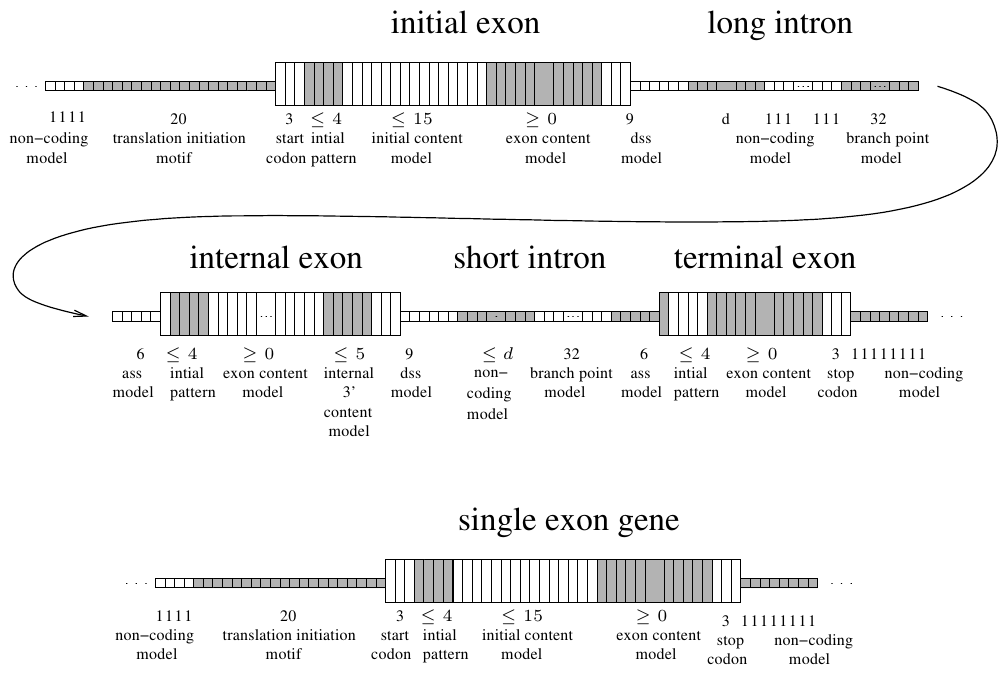
\includegraphics[width=8cm]{../pic/gene-structure.png}
\caption{真核基因结构}
\end{figure}
\end{frame}

%\begin{frame}{生物过程}
%\begin{figure}
%\centering
%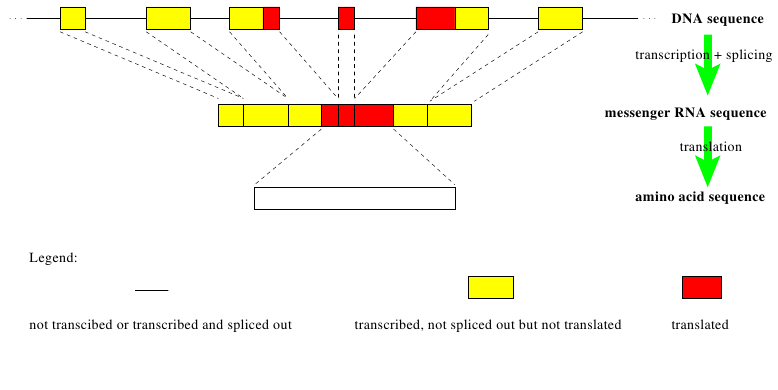
\includegraphics[width=10cm]{../pic/scheme-of-geneexpression.png}
%\caption{生物过程}
%\end{figure}
%\end{frame}

\begin{frame}{用复杂应对复杂}
与原核生物不同,真核生物基因结构复杂,不能用简单的马氏链方法预测。
复杂性体现在:
\begin{itemize}[<+->]
	\item 结构,强信号短特征 \alert<2>{-子模型作为隐状态}
	\item 大量噪声					 \alert<3>{-对intron,间区细致建模}
	\item 调控机制和表达模式 \alert<4>{-利用外部证据,可以做的地方}
\end{itemize}	
\end{frame}

\begin{frame}{用强模式构建隐状态}
\begin{block}{ 复杂不全是坏事:}
如果结构中某部分有强特征,则可以针对该特征建立细致的子模型。在整个augustus框架中,每个子模型是HMM的隐状态。
\end{block}
\begin{block} { 为什么不用HMM预测原核生物?}
1:原核基因相对均匀,没有强模式构建隐状态;2:状态间没有强依赖关系
\end{block}
\begin{block}{问题}
\alert{一阶HMM是在用非依赖的方法处理依赖问题?}马氏链或HMM,所谓马氏性质未必界限分明
\end{block}
\end{frame}

%------------------------------
\subsection{HMM简介}
\begin{frame}{真正的简介}
说三个算法,具体对HMM 的算法链到之前的HMM教程。
\end{frame}
\subsection{HMM in augustus}
\begin{frame}{HMM in augustus}
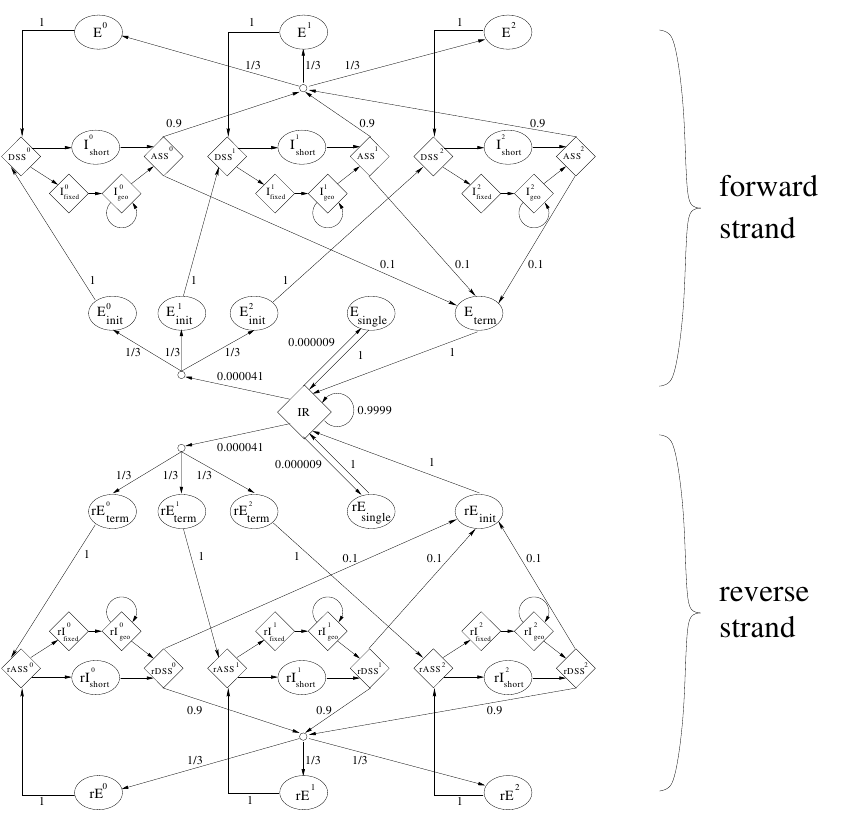
\includegraphics[height=13cm]{../pic/big-scheme.png}
\end{frame}

\begin{frame}{HMM in augustus}
\begin{itemize}
	\item 符号发射不定长,目标是寻找好的parse
	\item 多相位,2方向
\end{itemize}	
\end{frame}
%------------------------------------
\subsubsection{外显子建模}
\begin{frame}{外显子建模}
\begin{figure}
\centering
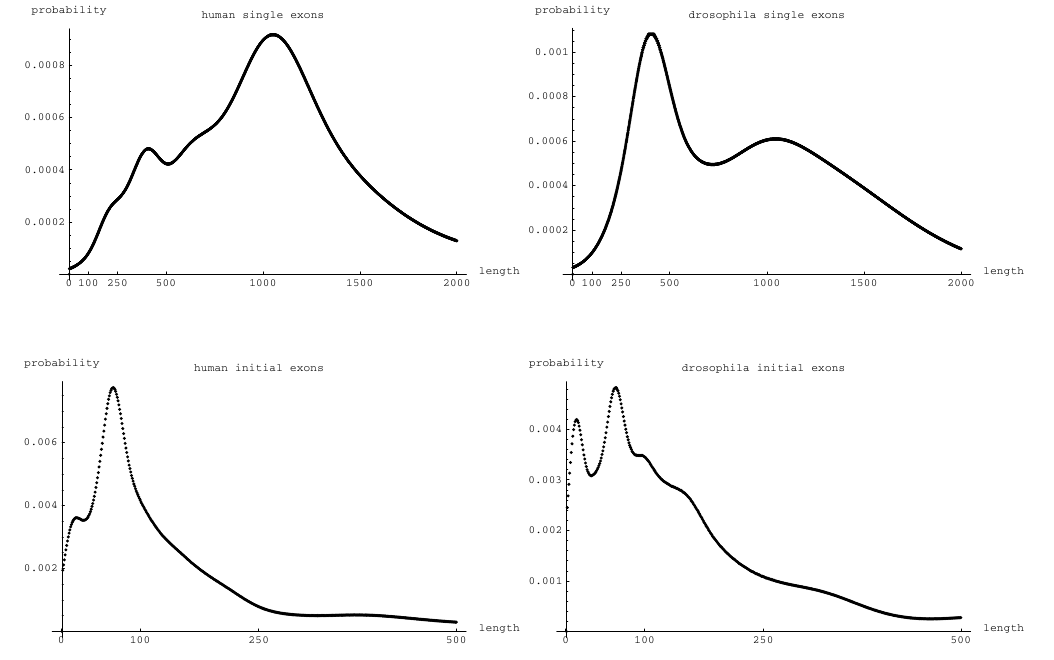
\includegraphics[width=10cm]{../pic/extron-length-1}
\caption{single and initial extron length distribution}
\end{figure}
\end{frame}

\begin{frame}{外显子建模}
\begin{figure}
\centering
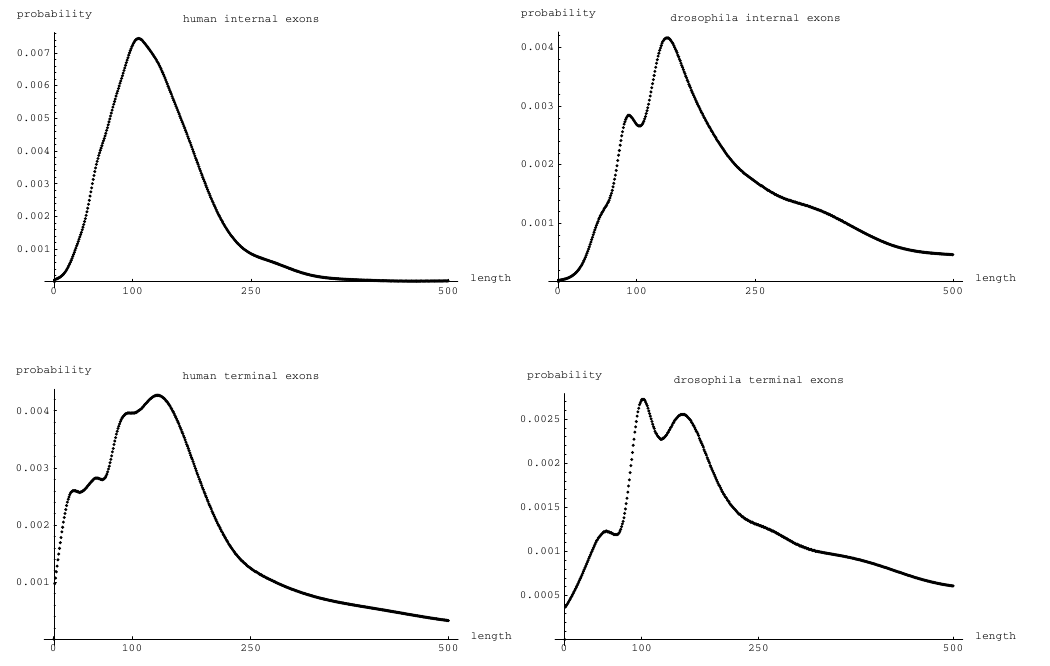
\includegraphics[width=10cm]{../pic/extron-length-2}
\caption{internal and terminal extron length distribution}
\end{figure}
\end{frame}

\begin{frame}{外显子建模}
\begin{itemize}
	\item  human: single, initial, internal, terminal:
	n = 462, n = 822, n = 4334, n = 822, respectively;
	\item Drosophila: single, initial, internal,
	terminal: n = 76, n = 324, n = 917, n = 324, respectively.
	\item 外显子分布窄,可以构造经验分布
	\item 密度估计利用高斯核函数
\end{itemize}	
\end{frame}
%------------------------------------
\subsubsection{内含子建模}
\begin{frame}{内含子建模}
\begin{figure}
\centering
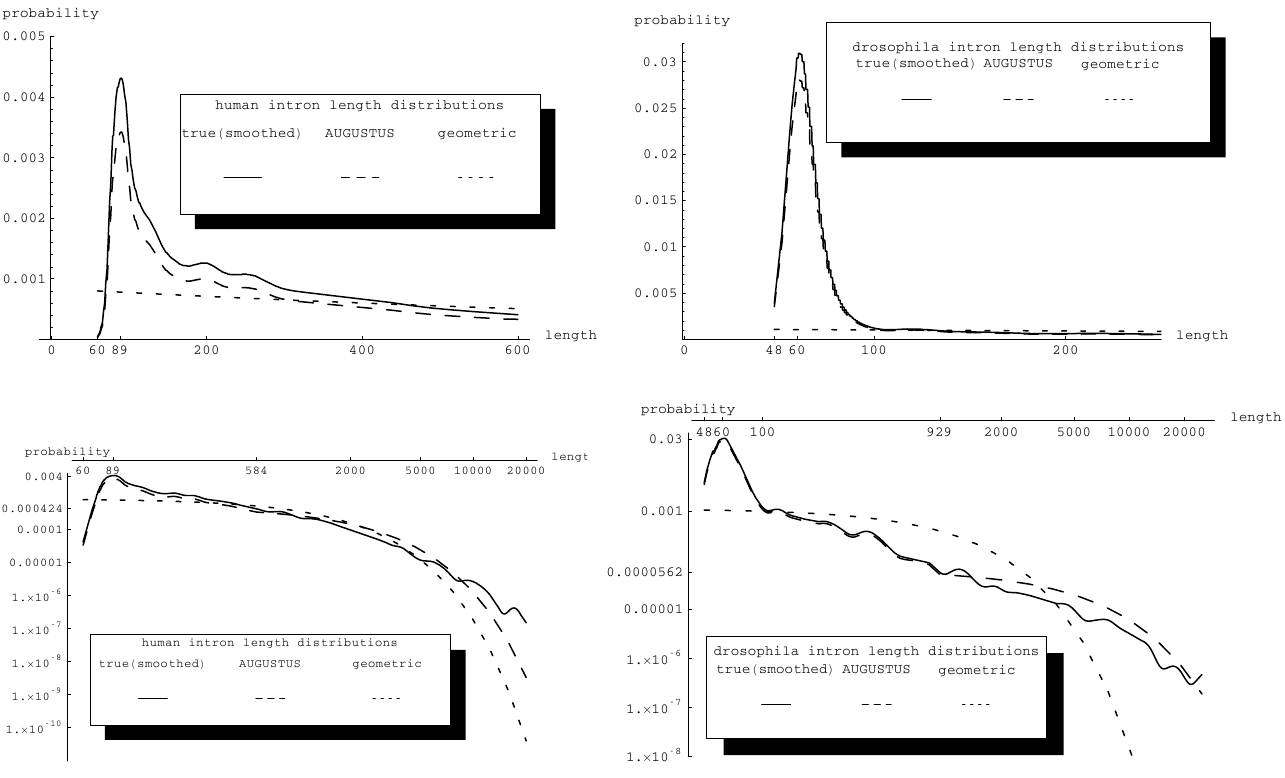
\includegraphics[width=10cm]{../pic/intron-length}
\caption{intron length distribution}
\end{figure}
\end{frame}

\begin{frame}{内含子建模}
显然:
\begin{itemize}[<+->]
	\item 内含子分布宽
	\item 内含子分布比外显子规律
	\item 峰后近似几何分布,对长内含子有低估,适当shift
\end{itemize}	
几何分布对内含子的低估问题:\alert{Reese et all,GENIE,a gene finder for Drosophila.}\\
\pause
所以:
\begin{itemize}
	\item 宽分布不适合采用经验分布描述(内存开销只是一方面)
	\item 采用经验分布+几何分布的混合模型,有shift,但没有验证是否解决了对长内含子的低估
\end{itemize}
\end{frame}

\begin{frame}{内含子建模}
\begin{figure}
\centering
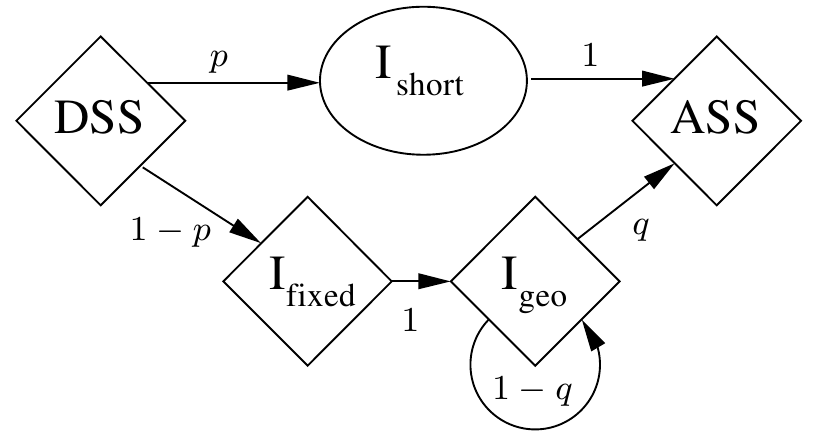
\includegraphics[width=10cm]{../pic/intron-model.png}
\caption{augustus 内含子模型}
\end{figure}
\begin{center}
\hyperlink{内含子参数确定}{\beamerbutton{内含子参数}}
是由三个限制条件决定的。
\end{center}
\end{frame}

%-------------------------------
\subsubsection{其他子模型}
\begin{frame}{强短信号}
真核基因结构复杂证据之一是在基因上下游有丰富的特征模体(\alert{motif}),有效识别这些模体可以帮助检测潜在基因区域。\\
除了对外显子和内含子长度建模外,augustus也对这些短模式建立子模型。
\begin{figure}
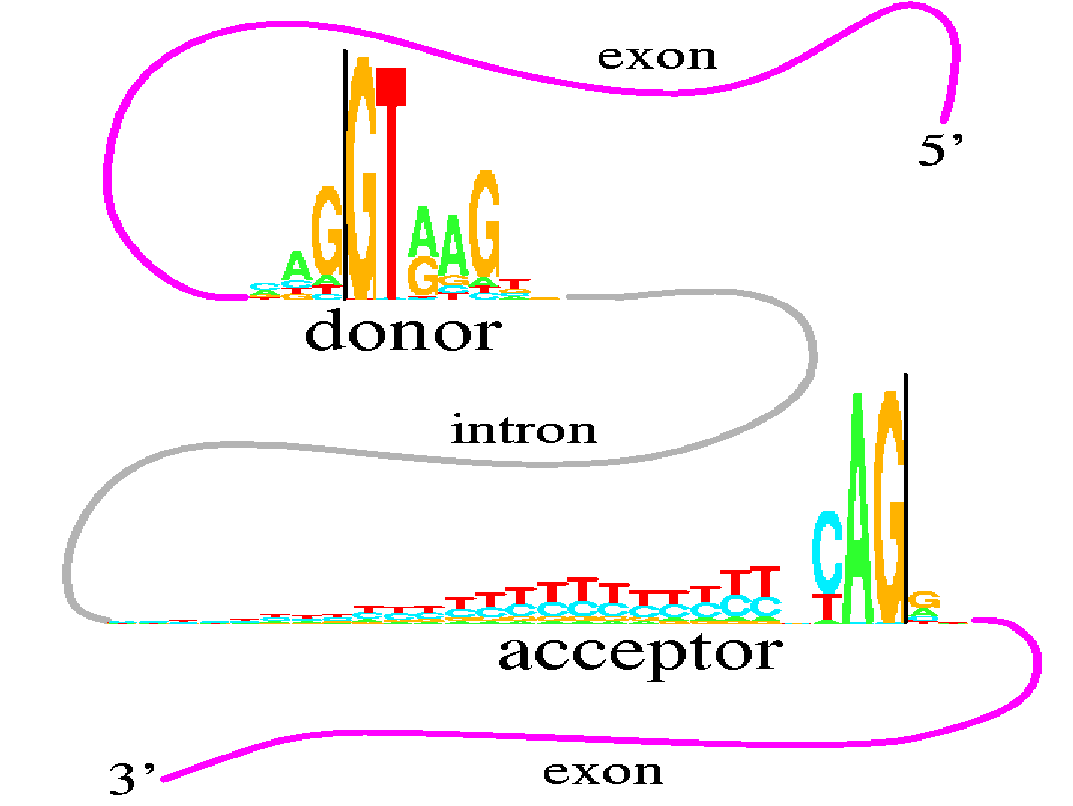
\includegraphics[width=6cm]{../pic/motif_GTAG}
\caption{外显子与内含子之间由GT-AG间隔,这是一个明显的短信号}
\end{figure}
这是比较强的一个模式: donor 7.9bits,acceptor 9.4bits\\
注意,所有这些模式都是在可靠比对的maf数据中训练得到的,信息含量的计算同样,仅在训练过程中有用。这些值在预测过程中都是非确定的。特别是一些很短模式,在未经可靠比对的情况下难以确定某一处高分位点是否只是偶然排列。
\end{frame}

\begin{frame}{两个滑动模型}
对子模型建模augustus采用原核基因预测常用的两个小模型:窗口加权字串模型(WWAM),插值马氏链(IMM)。\\
这两个模型的训练与原核基因的短模式训练相似。
\end{frame}

\begin{frame}[label=例子]{其他子模型}
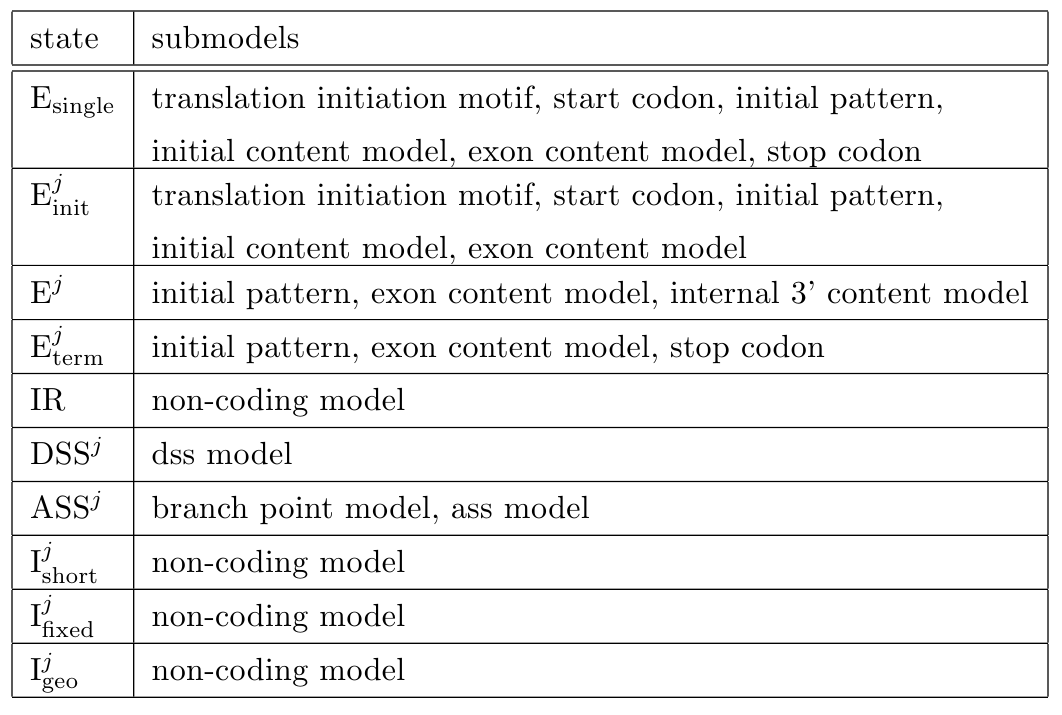
\includegraphics[width=10cm]{../pic/submodels}
\end{frame}

%-----------------------------
\subsubsection{转移矩阵}
\begin{frame}{转移矩阵}
以上定义的所有模型均为‘发射模型’,是HMM中的微观部分,以(条件)概率分布(矩阵)形式存在,保证打分规则一致性。另外,即使所有模型已经完整定义,在预测阶段,HMM沿未知序列滑动时,事先不知道parse是什么样,因此不能直接使用。\\
子模型之间的转移由转移矩阵决定,仍然是概率形式,是HMM的宏观部分。转移矩阵参数在:\alert{/augustus/config/model/}定义。\\
\end{frame}
\begin{frame}
\begin{columns}
	\begin{column}{5cm}
 constraints\_shadow\_partial.txt\\
 constraints\_shadow\_partial\_utr.txt\\
 states\_shadow\_2igenic.cfg\\
 states\_shadow.cfg\\
 states\_shadow\_intronless.cfg\\
 states\_shadow\_utr.cfg\\
 states\_singlestrand\_2igenic.cfg\\
 states\_singlestrand.cfg\\
	\end{column}
	\begin{column}{5cm}
 trans\_shadow\_atleastone.pbl\\
 trans\_shadow\_complete.pbl\\
 trans\_shadow\_complete\_utr.pbl\\
 trans\_shadow\_exactlyone.pbl\\
 trans\_shadow\_intronless.pbl\\
 trans\_shadow\_partial.pbl\\
 trans\_shadow\_partial\_utr.pbl\\
 trans\_singlestrand\_atleastone.pbl\\
 trans\_singlestrand\_complete.pbl\\
 trans\_singlestrand\_exactlyone.pbl\\
 trans\_singlestrand\_partial.pbl\\
	\end{column}
\end{columns}	
\\
一些模型变化可以在这里实现,比如*singlestrand*和*shadow*分别应用于单链和双链预测。
\end{frame}
%-------------------------------
\subsection{模型训练}
\begin{frame}{模型训练}
这里整理默认训练集参数,详细,周末更新
\end{frame}

%----------------------------
\subsection{模型的变体}
\begin{frame}{模型的变体}
\begin{columns}
\begin{colunm}{5cm}
geneModel=:\\
\beign{itemize}[<+->]
	\item partial(default)
	\item intronless
	\item complete
	\item atleastone
	\item exactlyone
\end{itemize}	
\begin{column}
	\item singlestrand=true
	\item hintsfile=hintsfile
	\item extrisnicCfgFile=cfgfile
	\item naxDBAOueceSuze=n
\end{frame}
%----------------------------
\subsection{基于GC 含量的训练}
\begin{frame}{GC content dependent training}
\begin{itemize}
\item Burge:基因预测模型的多数参数与GC含量关系密切。
\item Genescan 训练集分GC\%(<43\%,43\%-51\%,51\%-57\%,>57\%)4个子集训练4组参数,预测时根据输入序列GC含量选择其中一组参数。					
\end{itemize}
\end{frame}

\begin{frame}
Genescan 没有充分利用训练集。
\begin{itemize}
\item Mario:Augustus 将训练集按GC含量分成10份,用所有训练数据单独训练每个子集
\item 参与训练的子集权重由与被训练子集的平均GC含量($\alpha$)差异决定,权重决定训练层数
\item 权重近似成1-10之间的整数:$w(\alpha,\beta)=cell(10*exp(-200*(\alpha-\beta)^2))$
\item 在预测时,选择与输入序列GC含量接近的一组参数进行预测。
\item 权重参数文件在:$augustus/config/species/centain-species/certain-species\_weightmatrix.txt$\\
\item Pitfall:augustus每个子集的size?
\end{itemize}			
\end{frame}

%---------------------------
\subsection{利用外部证据推断基因结构}
\begin{frame}{外部证据}
这是最容易提升性能的部分,除了augustus,genescan等软件也在做这种努力。
整合外部hint的参数文件在:/augustus/config/extrinsic/**.cfg,主要规定了激励、罚分规则。
\begin{itemize}
				\item M manual anchor 
				\item P protein database hit
				\item E est database hit
				\item C combined est/protein database hit
				\item D Dialign
				\item R retroposed genes
				\item T transMapped refSeqs
\end{itemize}	
\end{frame}
%----------------------------
\subsection{augustus实现}
\begin{frame}{模块及变量介绍}
参考张磊的文档,关键参数文件确定
\end{frame}

%----------------------------
\section{用例测试}
\subsection{原核基因:Glimmer}
周末更新-刘耿加入
\begin{frame}{数据集}
\end{frame}
%----------------------------
\subsection{真核基因:Augustus}
周末更新-刘耿加入
\begin{frame}
\end{frame}

%----------------------------
\section{augustus要解决的问题}
\begin{frame}
以下问题是需要解决的:
\begin{itemize}
	\item 短模式训练400阈值是否合理
	\item GC训练加权是否考虑子集大小
	\item 怎么使用orf 
	\item 怎么整合外部数据(有文献,查代码)
\end{itemize}	
下一阶段的计划是在代码层面理解augustus。
\end{frame}
%-----------------------------
\section{补充材料}
\subsection{IMM 模型}
\begin{frame}[label=IMM frame]
\begin{block}{整体分值计算}
$$P(S|M)=\sum^{n}_{x=1or9}IMM_8(S_x)$$
\end{block}
\begin{block}{motif 分值计算}
$$IMM_k(S_x)={\lambda}_{k}(S_{x-1})*P_k(S_x)+[1-{\lambda}_{k}S_{x-1}]*IMM_{k-1}(S_x)$$
\end{block}								
$\lambda$是表示数据可信度的权数,$P_k(S_k)$是一个估计值。
\end{frame}

\begin{frame}{问题??}
整个序列打分有没overlap?\\
问题:\alert{随着阶数增加,$P_i(S_x)$的偏倚有没有变化?有迹可循吗?更进一步:权值确定是否考虑到如果阶数不同,对总体P贡献不同,在设计权值过程中有没考虑到怎样保证一致性?(后面的卡方定权值算是这种考虑的一部分,但只是局部,宏观层面的一致性更重要)预测应该是光滑的。WAMM模型有讨论?}
权值计算关键仍然是预测结果一致性的问题,似乎不是最好的方案,tradeoff吧
\end{frame}

%-----------------------
\subsection{ORF 确定基因结构}
\begin{frame}[label=ORF]{ORF}
完整的基因结构包含起始密码子和终止密码子:
\begin{itemize}
	\item A genome of length n is comprised of (n/3) codons
	\item Stop codons break genome into segments between consecutive stop codons
	\item The subsegments of these that start from the Start codon (ATG) are ORFs
\end{itemize}
如果序列是随机的,终止密码子应该每21($21=64/3$)个密码子中出现一次,基因长度要大于此长度。设定合理的阈值确定长ORF即可将随机序列与基因分离。
当确定一段orf后可以结合密码子使用偏倚,motif位点特征等进一步分析确定是否是基因。
\end{frame}
%-------------------------
\subsection{偏倚数量化}
\begin{frame}{偏倚数量化}
基因组在不同层面上存在组成偏倚。
\begin{itemize}[<+->]
	\item GC 含量 \pause 影响多数参数训练
	\pause
	\item 密码子	 
	\item 信号位点碱基丰度 \pause 检测短模式
\end{itemize}	
\end{frame}

\begin{frame}{偏倚数量化}
\begin{figure}
\centering
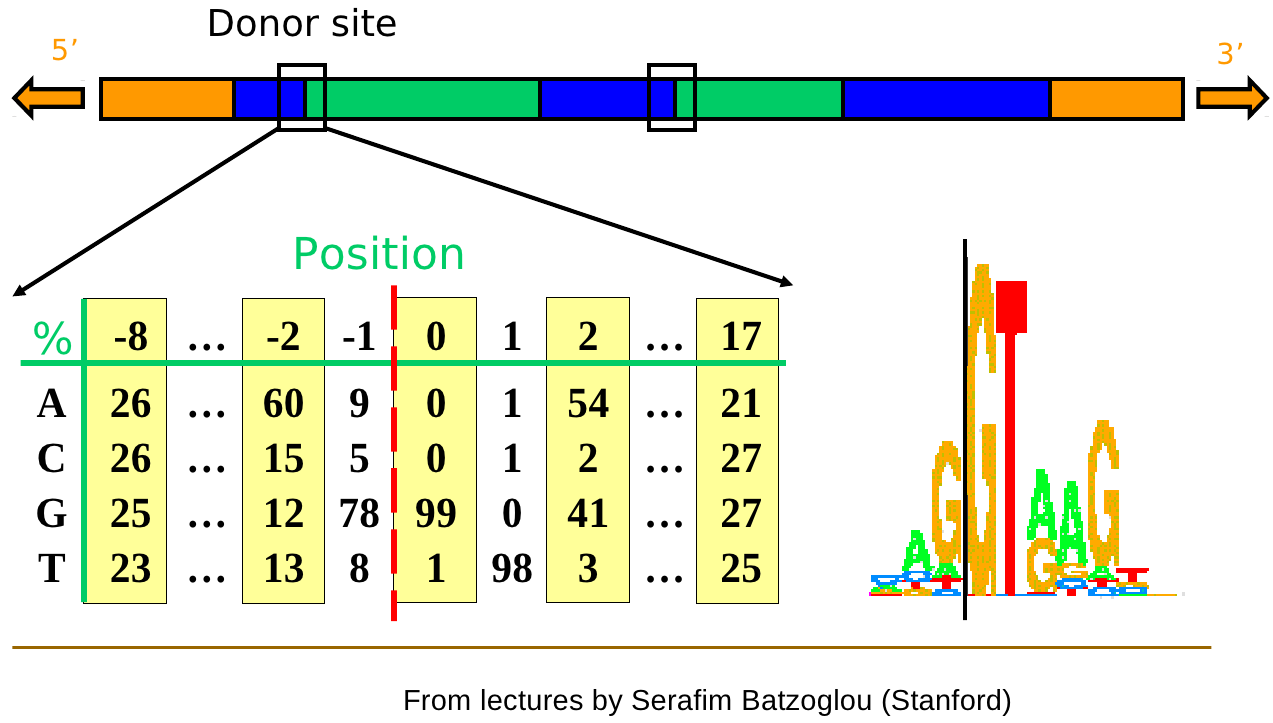
\includegraphics[width=10cm]{../pic/frequency-bias}
\caption{供体位点显示强烈偏倚}
\end{figure}
\end{frame}

\begin{frame}{偏倚数量化}
在真核基因预测中,我们关心的子模型特征通常是碱基丰度偏倚。对偏倚数量化既是统计依据的需要也便于程序自动工作。\\								
假定:
\begin{itemize}

\item 背景序列每个字出现概率是均匀分布(1/20 或 1/4)
	\item	强信号处概率分布是不均匀的(但无须知道具体分布)
\end{itemize}
\alert{一个好的数量标准可以反映这种差异,它最好是这二者的函数。}
\begin{block}{出于同样的工程需要,这个量已被信号工程师定义过:}
$H=-\sum^{4or20}_{i=1}P_i*(log_{2}Pi)$
\end{block}
%这个定义满足可加性,单调性,端点意义明确,几乎是完美定义。反映的是在某位点碱基丰度的不确定性。如果以背景频率作零假设构造LTR,则是交叉熵, 可以评估该点的信号强度(相对于背景)。\\
若以2为底取对数,信息强度的单位是bit。
\end{frame}

\begin{frame}{偏倚数量化}
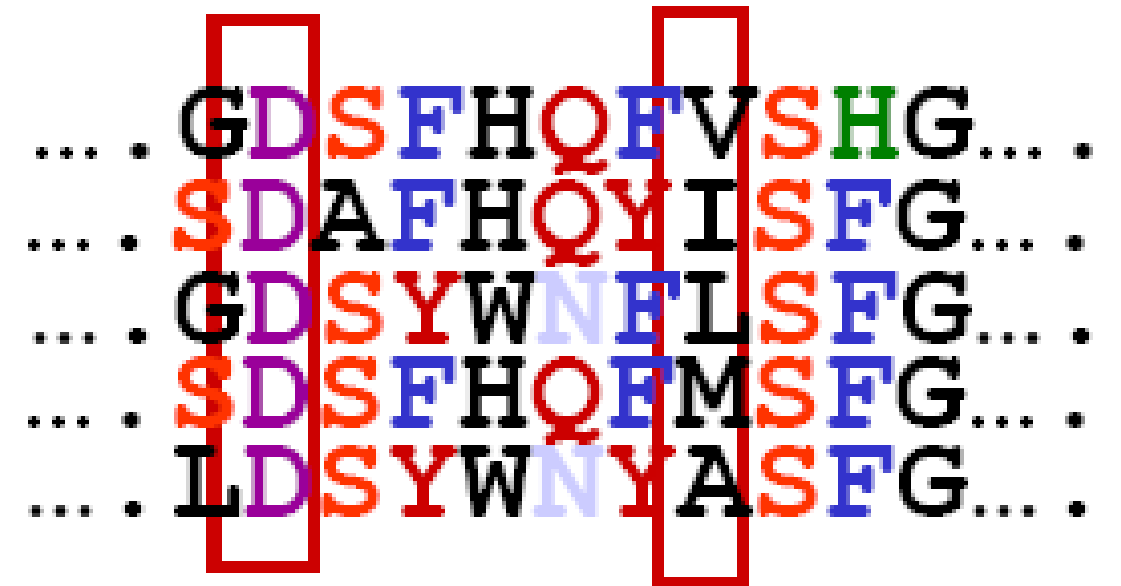
\includegraphics[width=8cm]{../pic/entropy_sample}
\begin{itemize}
\item 位点1:$H_{bg}=-\sum^{20}_{i=1}(1/20)*\log_{2}(1/20)=4.32bit,H_{site1}=0bit$,信号强度:4.32bit\\
\item 位点2:$H_{bg}=-\sum^{20}_{i=1}(1/20)*\log_{2}(1/20)=4.32bit,H_{site2}=4.32bit$,信号强度:0bit
\end{itemize}
\end{frame}
%--------------------------------------
\subsection{内含子参数确定}
\begin{frame}[label=内含子参数]{内含子参数确定}
内含子模型三个参数确定:
\begin{itemize}[<+->]
	\item $d+\frac{1}{q}=E[L]$
	\item $P(M=d)=P(M=d+1)$
	\item $P(M=l)=(1-p)(1-q)^{l-d-1}q$
\end{itemize}	
\end{frame}

\end{document}



